\documentclass[aps,prl,twocolumn,superscriptaddress,showpacs,floatfix,10pt]{revtex4-2}
\usepackage{amsmath,amssymb,graphicx,bm}
\usepackage[colorlinks=true,linkcolor=blue,citecolor=blue,urlcolor=blue]{hyperref}

\begin{document}

\title{Two-channel signatures of the \texorpdfstring{$E_7$}{E7} spectrum in a blockaded Rydberg chain}
\author{[Author]}
\affiliation{[Affiliation]}
\date{October 27, 2026}

\begin{abstract}
The thermal deformation of the tricritical Ising conformal field theory is an
integrable theory with seven $E_7$ particles. In a blockaded Rydberg chain, lattice
momentum separates its odd and even particles: a staggered detuning probe couples
to $\sigma$ and a uniform one to $\varepsilon$. Exact diagonalization of the
strictly blockaded chain with a $1/r^6$ tail, up to $L=36$, locates a
direction-dependent parameter region in which the four light particles
$A_1$--$A_4$ appear as two sharp peaks per channel, with gap ratios within
$3\%$ of $E_7$. This agreement changes by less than one percentage point across
the reported $1.7\%$ calibration uncertainty of the interaction. On open chains of
$19$--$27$ atoms, the four resonances are consistent with standing waves of the
bulk particles, with the largest deviation for $A_4$; a tapered drive suppresses $A_1$ and $A_2$ cross-channel leakage
below $0.03\%$, but leaves $7.5\%$ and $1.9\%$ for $A_3$ and $A_4$. The
shallow bound state $A_4$ carries the slowest finite-size corrections and sets the
resolution requirement. The heavy particles $A_5$--$A_7$ are not resolved.
\end{abstract}

\maketitle

\emph{Introduction.}---Relevant perturbations of a two-dimensional conformal
field theory (CFT) can produce integrable massive theories with spectra fixed by
exceptional Lie algebras. The magnetic perturbation of critical Ising theory
realizes $E_8$~\cite{Zamolodchikov1989}, with experimental signatures in
CoNb$_2$O$_6$~\cite{Coldea2010} and Rydberg arrays~\cite{Vovrosh2025}.
The leading thermal perturbation of the tricritical Ising (TCI) CFT, with central
charge $c=7/10$, instead realizes $E_7$~\cite{Christe1990,Fateev1990,Acerbi1996}.
Writing $r_a=m_a/m_1$, the seven ratios are
\begin{multline}
 (r_1,\ldots,r_7)=(1,\,1.2856,\,1.8794,\,1.9696,\,\phantom{)}\\
 2.5321,\,2.8794,\,3.7017).
 \label{eq:masses}
\end{multline}
with $\mathbb Z_2$ parities $(-,+,-,+,+,-,+)$ in the disordered
phase~\cite{Lepori2008}. An experimental identification of this spectrum remains
an open problem~\cite{Mussardo2022}.

Rydberg chains host Ising criticality, and an effective attraction produces a
tricritical point~\cite{Bernien2017,Slagle2021}. Sun \emph{et al.}~\cite{Sun2026}
reached it by preparing the upper edge of the blockaded sector, equivalent in the
projected model to an attractive ground-state problem, and measured finite-size
CFT spectra. This motivates spectroscopy of the neighboring gapped regime.

The field-theory inputs are established: the Rydberg density--CFT operator
correspondence~\cite{Slagle2021}, the $E_7$ form factors and selection
rules~\cite{Acerbi1996,CortesCubero2022}, and their threshold structure.
Kir\'aly and Lencs\'es~\cite{KiralyLencses2026} have also obtained lattice-quench
spectra compatible with the even particles $A_2,A_4,A_5$ in the Blume--Capel
chain, including form-factor amplitude comparisons. That study uses $A_2$ to
calibrate the mass scale; it does not independently resolve $A_1$.
Here we show that a Rydberg chain gives access to both parity sectors, so that
odd and even light particles can be compared on one platform. We map the
parameter region where four light peaks match $E_7$, identify the standing-wave
structure of open-chain resonances, and quantify the cross-channel leakage and
the finite-size constraint set by $A_4$.

\begin{figure*}[t]
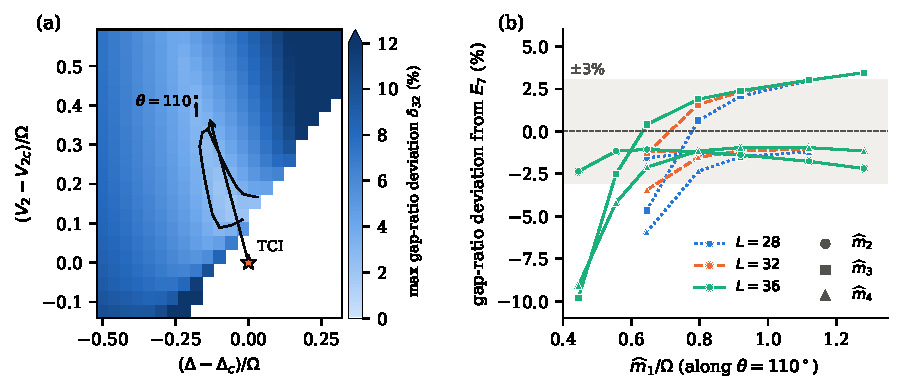
\includegraphics[width=0.95\textwidth]{fig1_window.pdf}
\caption{Finite-chain spectral matching region. (a) $\delta_L=100\max_{a=2,3,4}|(\widehat m_a/\widehat m_1)/r_a-1|$ at $L=32$;
the contour marks $3\%$. Grid spacings are $0.04\Omega$ in $\Delta$ and
$0.035\Omega$ in $V_2$. Blank cells fail the numerical filters
$L\widehat m_1/\Omega\ge18$ and $\widehat m_2\ge\widehat m_1/2$;
these filters do not establish phases or convergence.
The star estimates TCI; the arrow marks $\theta=110^\circ$.
(b) Individual gap-ratio deviations along that direction. Symbols identify the
candidate levels and line styles identify sizes. The band is $\pm3\%$; lines guide the eye.
Neither panel is an experimental error budget.}
\label{fig:window}
\end{figure*}

\emph{Model and field content.}---We study the projected Hamiltonian
\begin{equation}
 \begin{aligned}
 H={}&\sum_j\left[\frac{\Omega}{2}P_{j-1}X_jP_{j+1}-\Delta n_j\right]\\
    &+\sum_{i<j,\,d_{ij}\ge2}V_2(2/d_{ij})^6 n_i n_j.
 \end{aligned}
 \label{eq:H}
\end{equation}
with the constraint $n_jn_{j+1}=0$, $P_j=1-n_j$, and $V_2<0$.
The distance $d_{ij}$ is $|i-j|$ for open chains and the shortest distance on a
periodic chain; each pair is counted once. We set $\hbar=\Omega=a=1$, where $a$
is the lattice spacing. All allowed interaction pairs are retained within each
finite chain.

Equation~\eqref{eq:H} is the strict-blockade approximation to the sign-reversed
experimental problem, not the full experimental Hamiltonian. It omits the
finite-blockade correction $H_2$ of Ref.~\cite{Sun2026}, which contains diagonal
shifts and correlated hopping of order $\Omega^2/V_1$. We compute ground-state response
on open chains without boundary detuning.

In the long-wavelength theory, one-site translation exchanges the two density-wave
patterns and implements the internal $\mathbb Z_2$ together with spatial
translation~\cite{Slagle2021}. The density has the expansion
\begin{equation}
 n_j\simeq\bar n+c_\varepsilon\varepsilon+c_{\varepsilon'}\varepsilon'
       +(-1)^j(c_\sigma\sigma+c_{\sigma'}\sigma')+\cdots .
 \label{eq:dens}
\end{equation}
Thus zero-momentum even particles occur near lattice momentum $0$, and odd
particles near $\pi$. This identification uses bulk translation symmetry; open-chain
reflection parity is a different quantum number.

Both $\Delta$ and $V_2$ generate the even relevant perturbations
$g_\varepsilon\varepsilon+g_{\varepsilon'}\varepsilon'$, with RG eigenvalues
$9/5$ and $4/5$. For a straight path of distance $t$ from TCI with a nonzero
linear component in $g_\varepsilon$,
\begin{equation}
 \eta=\frac{g_{\varepsilon'}}{|g_\varepsilon|^{4/9}}
       \propto t^{5/9},\qquad m_1\propto t^{5/9}.
 \label{eq:RG}
\end{equation}
On the disordered side such paths approach the thermal $E_7$ theory as $t\to0$
if the system size is increased simultaneously. The growing correlation length
limits this approach at fixed $L$. We have not calibrated the map from lattice
parameters to $(g_\varepsilon,g_{\varepsilon'})$; a region of small mass-ratio
errors need not identify the pure thermal trajectory or separate competing corrections.

\emph{Probes and numerical method.}---For a periodic ground state, the connected
density response is
\begin{equation}
 S_k(\omega)=\frac1L\sum_{n\ne0}
 \left|\left\langle n\left|\sum_j e^{ikj}n_j\right|0\right\rangle\right|^2
 \delta[\omega-(\mathcal E_n-\mathcal E_0)].
 \label{eq:spec}
\end{equation}
Uniform and staggered probes select $k=0$ and $\pi$ exactly. In the $E_7$ limit,
Eq.~\eqref{eq:dens} couples them principally to $\varepsilon$ and $\sigma$,
respectively. The proposed $k=\pi$ coupling to $\sigma$ already appears in
Ref.~\cite{Sun2026}. For a pure continuum operator $\mathcal O$, one-particle
weights obey $w_a\propto|F_a^{\mathcal O}|^2/m_a$. Known form factors give
$w_3/w_1=0.067$, $w_6/w_1=0.0030$ for $\sigma$, and
$w_4/w_2=0.143$, $w_5/w_2=0.038$, $w_7/w_2=0.0012$ for
$\Theta\propto\varepsilon$~\cite{Acerbi1996,CortesCubero2022}.
Absolute interchannel amplitudes are not universal.

We use sparse exact diagonalization in the constrained space for periodic
$L\le36$ and open $L=19,23,27$. Spectra use reorthogonalized Lanczos iterations
(up to 400 for the periodic spectra and 250 for the open spectra shown).
Small-system checks compare momentum-sector energies and weights with full-space
diagonalization to numerical precision. They do not establish convergence of the
large-system continuum.

We denote the first two gaps in the $k=\pi$ sector by
$\widehat m_1(L),\widehat m_3(L)$ and the first two excited gaps at $k=0$ by
$\widehat m_2(L),\widehat m_4(L)$. These are candidate light-particle levels,
not independently extrapolated masses. Throughout the parameter scan, the labels
follow energy ordering within each sector. For open chains, $\omega_a^{\rm o}$
denotes a candidate resonance energy selected by its dominant probe weight.

Simultaneous crossings of $L$ times the lowest odd and lowest excited even gaps
locate a finite-size TCI estimate. The $L=28/32$ crossing gives
$(\Delta_c,V_{2c})=(-1.5011,-1.6260)$, within $10^{-3}$ of the $24/28$ estimate
and close to the experimental calibration~\cite{Sun2026}.
Fixing $v\simeq1.90$ using $x_\sigma=3/40$ gives other rescaled gaps near
$0.875$ at $k=\pi$, and $0.198,1.18$ at $k=0$, consistent with
$x_{\sigma'}=7/8$, $x_\varepsilon=1/5$, $x_{\varepsilon'}=6/5$.
The value of $x_\sigma$ is an input to this comparison.

\begin{figure}[htbp]
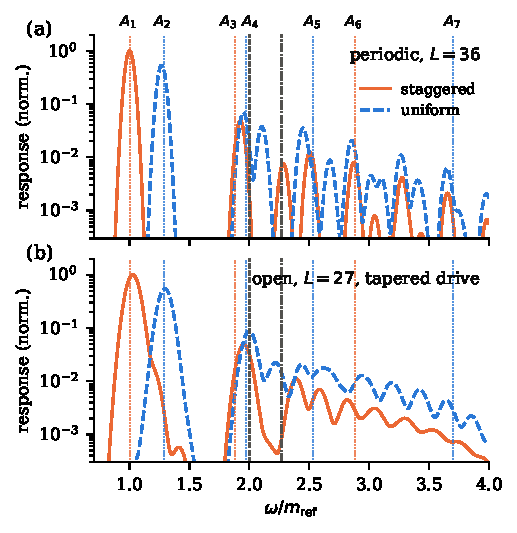
\includegraphics[width=\columnwidth]{fig2_spectra.pdf}
\caption{Response at Eq.~\eqref{eq:point}: (a) periodic $L=36$, without size
averaging; (b) open $L=27$ with a $\sin^2$ drive envelope. Both use
$m_{\rm ref}=\widehat m_1(36)=0.9196\Omega$ and are normalized to their own
staggered peak height. Solid orange: staggered; dashed blue: uniform.
Only (a) has exact momentum selection. Gaussian standard deviations
$0.03m_{\rm ref}$ and $0.05m_{\rm ref}$ illustrate smoothing, not instrumental
linewidths. Dotted lines mark ideal $E_7$ ratios. Gray dashed/dash-dotted lines
mark $2m_{\rm ref}$ and $m_{\rm ref}+\widehat m_2(36)$: periodic-gap sums,
not measured open-chain continuum edges.}
\label{fig:spec}
\end{figure}

\emph{Matching region and finite size.}---We scan
$(\Delta,V_2)=(\Delta_c,V_{2c})+t(\cos\theta,\sin\theta)$.
Figure~\ref{fig:window} identifies a finite region of small errors among the
three gap ratios. Along $\theta=110^\circ$, the sampled $L=36$ points at
$t=0.1,0.15,0.2$ have maximal errors below $3\%$; at $t=0.3$ the maximum is
$3.01\%$. Nearby directions $90^\circ$ and $130^\circ$ also contain matching
points. In contrast, the sampled $\theta=180^\circ$ points never reach $5\%$
accuracy; deviations near $210^\circ$ can reach $10$--$25\%$.
This direction dependence concerns the accessible finite-chain window and does
not contradict the generic asymptotic limit in Eq.~\eqref{eq:RG}.

At $\theta=110^\circ,t=0.2$, corresponding to
$(\Delta,V_2)=(-1.5695,-1.4381)$, we find
$\widehat m_1(36)=0.9196\Omega$ and
\begin{equation}
 \frac{(\widehat m_2,\widehat m_3,\widehat m_4)}{\widehat m_1}
 =(1.2678,\,1.9243,\,1.9508).
 \label{eq:point}
\end{equation}
The relative deviations are $(-1.39,+2.39,-0.95)\%$.
At $t=0.1$, however, $\widehat m_3/\widehat m_1$ changes from $1.792$ to
$1.887$ between $L=28$ and $36$, illustrating the limitation closer to TCI.
At $t=0.3$ the three ratios change by less than $0.24\%$ over those sizes,
but this comparison is not an infinite-volume extrapolation.

The shallow $A_4$ bound state requires particular care. In the integrable theory,
$A_4$ occurs in the $A_1A_1$ scattering channel, with
\begin{equation}
 \mu_{11}^{4}=\sqrt{m_1^2-m_4^2/4}
             =m_1\sin(\pi/18)\simeq0.174m_1.
 \label{eq:mu}
\end{equation}
Its finite-volume energy can receive a leading bound-state correction
proportional to $e^{-\mu_{11}^{4}L/v}$, not simply
$e^{-m_1L/v}$~\cite{Pozsgay2008,CortesCubero2022}.
With the working gap and $v\simeq1.90$, the $E_7$ value of $\mu_{11}^4$ gives
$v/\mu_{11}^{4}\simeq12$ sites; the binding measured on the chain gives
$\simeq9$ sites. Both exceed $v/m_1\simeq2$ sites considerably.
In the data, $\widehat m_4/\widehat m_1$ changes from $1.9400$ to $1.9508$
between $L=28$ and $36$: only $0.56\%$ of its value, but $22\%$ of the latter
binding-energy estimate $2\widehat m_1-\widehat m_4$.
A mass-ratio tolerance alone therefore does not control near-threshold binding.

At the working point, the periodic weight ratios are $w_4/w_2=0.129$ and
$w_3/w_1=0.0483$. Mixing with $\sigma'$ contributes an effective relative
amplitude proportional to $(c_{\sigma'}/c_\sigma)(m_1a/v)^{4/5}$ at fixed CFT
normalization, since $x_{\sigma'}-x_\sigma=4/5$. The weights also contain
interference, finite-size, and nonintegrable corrections. We do not isolate these
sources or treat the pure-field ratios as precise lattice predictions.

\emph{Spectra and boundaries.}---The periodic response in
Fig.~\ref{fig:spec}(a) has two prominent subthreshold peaks in each sector,
consistent with the four candidate levels in Eq.~\eqref{eq:point}.
Momentum selection is exact. The next visible even-sector level at $L=36$ is
at $2.105m_{\rm ref}$, so its separation from the $A_4$ candidate is
$0.154m_{\rm ref}$, appreciably larger than the gap to the kinematic reference
$2m_{\rm ref}$. Discrete scattering levels can thus make a small-system spectrum
appear more separated than its infinite-volume counterpart.

For open chains we use $O_{f,q}=\sum_j f_j e^{iqj}n_j$, where $q=0,\pi$ labels
the drive pattern rather than an exact momentum sector. Spectral weights are
normalized by $\sum_j f_j^2$. We compare $f_j=1$ with
$f_j=\sin^2[\pi(j+1)/(L+1)]$, $j=0,\ldots,L-1$.
At $L=27$, the latter gives dominant candidate resonance ratios
\begin{equation}
 (\omega_2^{\rm o},\omega_3^{\rm o},\omega_4^{\rm o})/\omega_1^{\rm o}
 =(1.2612,\,1.9030,\,1.9488),
 \label{eq:open}
\end{equation}
with $\omega_1^{\rm o}=0.9438\Omega$, within $2\%$ of $E_7$. The open-chain
energies are shifted upward by the lowest standing-wave momentum. With
$E_a(n)=\{\widehat m_a^2+[n v\pi/(L+1)]^2\}^{1/2}$, $v=1.90$, and the periodic
$L=36$ masses, the $n=1$ prediction reproduces $\omega_1^{\rm o}$ to $0.02\%$
and $\omega_{2,3}^{\rm o}$ to better than $0.8\%$ at $L=27$. The largest
deviation occurs for $A_4$: $1.8\%$, $2.9\%$, and $5.2\%$ at $L=27$, $23$, and
$19$. This size dependence is consistent with $A_4$ having the largest spatial
extent, as estimated above.

Table~\ref{tab:leakage} reports all four channel leakages, defined as the
integrated weight at the same candidate eigenenergy in the unintended probe
divided by its weight in the intended probe. At $L=27$, tapering reduces the
$A_1$ leakage from $0.149\%$ to $0.0267\%$, but the $A_3$ leakage only from
$9.22\%$ to $7.46\%$, and the $A_4$ leakage increases from $1.41\%$ to $1.94\%$.
Tapering therefore does not separate all sectors uniformly; at $L=19$, two
nearby uniform resonances also share substantial weight.
The strongest satellite, at $1.160\,\omega_1^{\rm o}$ for $L=27$, is the $n=3$
standing wave of $A_1$: under a flat drive, $(L+1)(E^2-\widehat m_1^2)^{1/2}$
equals $16.6$, $16.4$, and $16.6$ at $L=19$, $23$, and $27$, about $2.7$--$2.8$
times the $n=1$ value. The ratio below three is consistent with lattice-dispersion
curvature at this momentum. A flat drive gives it $9$--$13\%$ of the $A_1$ weight,
roughly as expected from its overlap with a uniform profile, and tapering reduces
this to $1.7\%$ at $L=27$. Its origin is thus bulk $A_1$, not a boundary bound state.

\begin{table}[htbp]
\caption{Leakage ratios in percent for tapered open-chain probes at the working
point. The intended probe is staggered for $A_1,A_3$ and uniform for $A_2,A_4$.
Labels denote finite-chain candidates.}
\label{tab:leakage}
\begin{ruledtabular}
\begin{tabular}{ccc}
Candidate & $L=27$ & $L=19$ \\
\hline
$A_1$ & $0.0267$ & $0.228$ \\
$A_2$ & $0.0192$ & $4.53$ \\
$A_3$ & $7.46$ & $39.4$ \\
$A_4$ & $1.94$ & $8.98$
\end{tabular}
\end{ruledtabular}
\end{table}

\emph{Thresholds and unresolved heavy particles.}---In the integrable,
translation-invariant theory, the lowest even and odd two-particle thresholds
are $2m_1$ ($A_1A_1$) and $m_1+m_2$ ($A_1A_2$). The exact $E_7$ scattering
amplitudes and form factors imply responses proportional to
$(\omega-2m_1)^{1/2}$ and $(\omega-m_1-m_2)^{-1/2}$ in the corresponding
channels~\cite{CortesCubero2022}. Here $S_{11}(0)=-1$ forces the identical-particle
form factor to vanish, whereas the relevant $A_1A_2$ form factor is nonzero at
threshold. These are integrable-limit predictions for the matrix-element-weighted response.

At our working point, the next odd-sector spectral level above the two light
peaks moves from $2.340\widehat m_1$ at $L=18$ to $2.284\widehat m_1$ at $L=36$,
toward the gap sum $1+\widehat m_2/\widehat m_1=2.268$.
The corresponding even-sector sequence moves from $2.296\widehat m_1$ at $L=24$
to $2.105\widehat m_1$ at $L=36$. This is consistent with the two different onsets, but does not determine
threshold exponents; on open chains, residual weight remains above $A_3$.

We do not resolve $A_5,A_6,A_7$. In the $E_7$ theory their masses lie above
allowed thresholds in their own sectors: $A_5,A_7$ above $2m_1$, and $A_6$ above
$m_1+m_2$. Nonintegrable perturbations can open decay channels such as
$A_5\to A_1A_1$ and $A_6\to A_1A_2$~\cite{Lepori2008}.
Across $L=18$--$36$ at $\theta=110^\circ$, $t=0.2,0.3$, the higher spectra do
not provide a stable heavy-particle assignment by energy and weight.
Finite chains do not measure decay widths, so this neither establishes nor
excludes heavy resonances in larger systems.

\emph{Experimental requirements.}---The protocol prepares a state near
Eq.~\eqref{eq:point} with the demonstrated TCI preparation~\cite{Sun2026}, applies
weak tapered uniform and staggered modulations, and compares the two responses.
The sign-changing staggered drive needs the two-color ($515$ and $813$ nm) tweezer
scheme proposed in Ref.~\cite{Sun2026}, beyond the one-color light shifts used so far.

Spectral resolution is especially consequential for $A_4$. The finite-chain
estimate $2\widehat m_1-\widehat m_4\simeq0.049m_{\rm ref}$ is about
$2\pi\times0.25$ MHz for $\Omega=2\pi\times5.5$ MHz; in ideal $E_7$ the relative
binding is smaller, $0.0304m_1$.
The illustrative open-chain broadening in Fig.~\ref{fig:spec} has
$\mathrm{FWHM}=2\sqrt{2\ln2}\,\sigma=0.118m_{\rm ref}$, about
$2\pi\times0.60$ MHz. Separating $A_4$ from the continuum therefore needs a linewidth below this
scale; the $E_7$ threshold suppression of the $A_1A_1$ response would help in the
scaling regime. Because of open-chain mixing, $A_3$ and $A_4$ should be assigned
by comparing both probes rather than by channel label alone.

The reported $1.7\%$ uncertainty in $V_2$~\cite{Sun2026} amounts to about
$0.028\Omega$. At $\Delta\simeq-1.60\Omega$, the $3\%$ region of
Fig.~\ref{fig:window}(a) extends over at least $0.14\Omega$ in $V_2$. Near the
working point, $\delta_{32}$ changes by at most $0.7$ percentage points per
$V_2$ grid step and $0.9$ per $\Delta$ step. Calibration errors of this size
therefore move the gap ratios by less than one percentage point in this criterion.

Finite-blockade corrections, preparation, decoherence, and readout are not
modeled; they must be included before the four-peak signature is used as an
experimental identification.

\emph{Conclusion.}---Because one-site translation implements the tricritical
$\mathbb Z_2$, a Rydberg chain can resolve both parity sectors of the $E_7$
spectrum with uniform and staggered probes. In the strictly blockaded model, we find
a direction-dependent region where four light particles appear as two peaks per
channel at $E_7$ ratios within $3\%$. This agreement is stable against the
reported interaction calibration uncertainty. Open-chain resonances follow the bulk
masses through standing-wave dispersion; a tapered drive suppresses the dominant
satellites, but channel mixing remains particle dependent. The shallow bound state
$A_4$ sets the most demanding finite-size and resolution requirements; the heavy
particles remain open. These results specify where to look and which systematics decide an observation.

\begin{acknowledgments}
[Acknowledgments.]
\end{acknowledgments}

\begin{thebibliography}{99}
\bibitem{Zamolodchikov1989}
A.~B. Zamolodchikov, Int. J. Mod. Phys. A \textbf{4}, 4235 (1989).
\bibitem{Coldea2010}
R.~Coldea, D.~A. Tennant, E.~M. Wheeler, E.~Wawrzynska, D.~Prabhakaran,
M.~Telling, K.~Habicht, P.~Smeibidl, and K.~Kiefer, Science \textbf{327}, 177 (2010).
\bibitem{Vovrosh2025}
J.~Vovrosh, J.~de~Hond, S.~Juli\`a-Farr\'e, J.~Knolle, and A.~Dauphin,
arXiv:2506.21299.
\bibitem{Christe1990}
P.~Christe and G.~Mussardo, Nucl. Phys. B \textbf{330}, 465 (1990).
\bibitem{Fateev1990}
V.~A. Fateev and A.~B. Zamolodchikov, Int. J. Mod. Phys. A \textbf{5}, 1025 (1990).
\bibitem{Acerbi1996}
C.~Acerbi, G.~Mussardo, and A.~Valleriani, Int. J. Mod. Phys. A \textbf{11}, 5327
(1996).
\bibitem{Lepori2008}
L.~Lepori, G.~Mussardo, and G.~Zs. T\'oth, J. Stat. Mech. (2008) P09004.
\bibitem{Mussardo2022}
G.~Mussardo, \emph{2D Ising model and its tricritical version: when theory meets
experiments}, lecture at IH\'ES (2022).
\bibitem{Bernien2017}
H.~Bernien \emph{et al.}, Nature \textbf{551}, 579 (2017).
\bibitem{Slagle2021}
K.~Slagle, D.~Aasen, H.~Pichler, R.~S.~K. Mong, P.~Fendley, X.~Chen, M.~Endres,
and J.~Alicea, Phys. Rev. B \textbf{104}, 235109 (2021).
\bibitem{Sun2026}
X.~Sun, Y.~Le, S.~Naus, R.~B.-S. Tsai, L.~R.~B. Picard, S.~Murciano, M.~Knap,
J.~Alicea, and M.~Endres, Nature \textbf{657}, 98--106 (2026).
\bibitem{CortesCubero2022}
A.~Cort\'es Cubero, R.~M. Konik, M.~Lencs\'es, G.~Mussardo, and G.~Tak\'acs,
SciPost Phys. \textbf{12}, 162 (2022).
\bibitem{KiralyLencses2026}
C.~Kir\'aly and M.~Lencs\'es, SciPost Phys. \textbf{20}, 030 (2026).
\bibitem{Pozsgay2008}
B.~Pozsgay, Nucl. Phys. B \textbf{802}, 435--457 (2008).
\end{thebibliography}
\end{document}
